\documentclass[a4paper]{usiinfbachelorproject}

\captionsetup{labelfont={bf}}
%%%%%%%%%%%%%%%%%%%%%%%%%%%% PACKAGES %%%%%%%%%%%%%%%%%%%%%%%%%%%%%
\usepackage{float}
\usepackage{amsmath}
\usepackage{subfig}
\usepackage{graphicx}
\usepackage{svg}

%%% Main Body %%%

\author{Sasha Toscano}

\title{\textbf{Understanding arbitrary code
execution}}
\subtitle{A case study on Pokémon Emerald}
\versiondate{\today}

\begin{committee}
%With more than 1 advisor an error is raised...: only 1 advisor is allowed!
\advisor[Universit\`a della Svizzera italiana, Switzerland]{ }{Carlo Alberto}{Furia}
%You can comment out  these lines if you don't have any assistant
\coadvisor[Universit\`a della Svizzera italiana, Switzerland]{ }{Marc}{Langheinrich}

\end{committee}

\abstract {
This thesis presents a case study of a real-world arbitrary code execution (ACE) exploit targeting Pokémon Emerald, a Game Boy Advance title, to explore the mechanics and implications of code reuse vulnerabilities on constrained platforms. By manipulating the game’s memory and control flow through crafted input, the attack achieves code execution without injecting new instructions, highlighting how even legacy systems without modern protections can be coerced into executing attacker-controlled behavior.

To frame this case within a broader context, the thesis also surveys complementary defensive approaches about detection and prevention of ACE and ACE-like exploits. The first is vulnerability detection through deep learning, specifically using Long Short-Term Memory (LSTM) networks trained to identify remote code execution patterns in PHP source code. The second approach focuses on mitigation techniques at the compiler level, reviewing G-Free, a strategy for eliminating exploitable return instructions, and EC-CFI, a control-flow integrity system that enforces strict validation of all indirect control transfers.

By combining the practical analysis of a concrete exploit with a review of contemporary defense strategies, this thesis illustrates the evolution of software exploitation and protection. It concludes by reflecting on the potential synergy between detection and mitigation techniques, and the relevance of compiler-based defenses even in low-level environments such as handheld gaming systems. 
\\
\textbf{Keywords}: Arbitrary Code Execution, Software Security, Compiler-Based Security, Pokémon Emerald, Vulnerability Detection, Vulnerability Prevention

}
\begin{document}
\maketitle
\tableofcontents\newpage
%\listoffigures\newpage

\section{Introduction}
In the world of software, security is one of the most critical concepts as it is the foundation of trust in the tools we use every day. Let it be something as simple as our browser remembering our passwords, or as complex as a bank's online banking system, we need to be able to trust that the programs we use are secure and that our data is safe and well protected. This is especially important in this day and age where we rely on these types of software for everything: from communication, to banking, and even to entertainment.

The software we use is often complex and interconnected, making it difficult to distinguish what is secure and what isn't. In many cases, these programs are often developed quickly and with limited resources, and as a result, security is often an afterthought in the development process, leading to oversights or the introduction of vulnerabilities that can be exploited by attackers.

One of the most common types\footnote{https://www.sciencedirect.com/topics/computer-science/arbitrary-code-execution} of these vulnerabilities is ACE, which allows a malicious unauthorized user to execute some arbitrary code on a target system or in a specific application. This can happen because software or computer systems in general are not capable of differentiating between some generic text and actual commands, without some proper protections put in place.

This then becomes a significantly serious issue as it can lead to unauthorized access to sensitive information, data loss, and even complete system compromise. These types of ACE vulnerabilities can be found in a wide range of software: including operating systems, web applications, and even video games. In fact, some of the most interesting ACE vulnerabilities have been found in video games like \textit{Super Mario World}\footnote{https://arstechnica.com/gaming/2014/01/how-an-emulator-fueled-robot-reprogrammed-super-mario-world-on-the-fly/}, where they have been used to allow users to literally "program" new games into the system to be played.

In this thesis, we will explore the concept of ACE using a case study of the game \textit{Pokémon Emerald} (2004) to demonstrate how such vulnerabilities can be exploited. We will then examine the current state of ACE-related attacks and discuss modern techniques that can be used to mitigate them. We will also look at some of the most common techniques used to protect against these vulnerabilities, and how they can be prevented.

\section{Arbitrary code execution}
\label{sec:ace}
I'd like to start with a simple explanation of what arbitrary code execution is: \textit{updog}. \\ And what is updog, you may ask? \textit{Not much, what's up with you?}

\begin{figure}[h!]
	\center{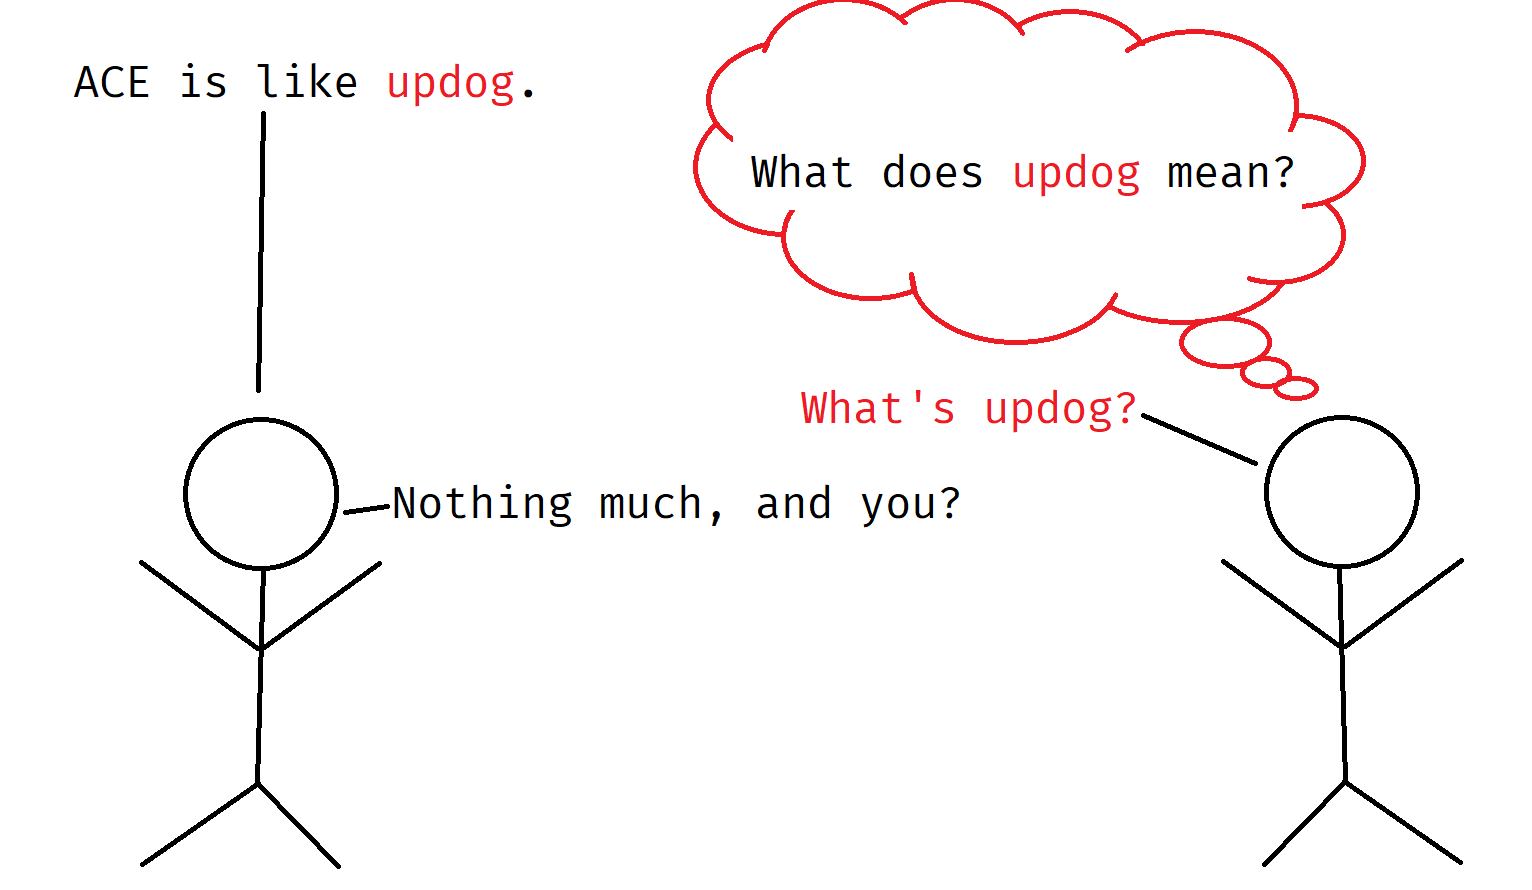
\includegraphics[scale=0.3]
		{figures/ace.png}}
	\caption{A graphical illustration of the \textit{updog} joke\label{fig:updog}}
\end{figure}

This joke, illustrated in figure \ref{fig:updog} (credits to Smoovers\footnote{https://www.youtube.com/watch?v=-XmXYCXX7y4}) is an extremely simple but direct way of explaining what ACE is. In this case the joke is self-explanatory, but the idea behind it is that we end up saying something (\textit{"what's up dawg?"}) that is not what we intended to say (\textit{"what does updog mean?"}). This is extremely similar to what happens during ACE in the real world, where the system ends up executing code that we did not intend to execute, albeit with dramatically more complicated consequences.

To get a bit more into the proper definition of things: ACE is a type of flaw or vulnerability that allows an attacker to execute some generally speaking malicious (or at least unauthorized) code on a target system\footnote{https://www.okta.com/identity-101/arbitrary-code-execution/}. Without proper protections and preventions put in place, an attacker can easily exploit these to gain access to sensitive information, take control of the system, or even cause damage to the system itself. The severity of this incidents can vary greatly: in the past these exploits have gone from something low-level like allowing gamers to better their speedrunning performances\footnote{https://www.youtube.com/watch?v=A2DlyLPr4Ws} (where speedrunning is the art of playing a video game with the goal of completing it as fast as possible), to something a fair bit more complicated, like leaking sensitive kernel memory on real world systems, as was the case in Retbleed\footnote{https://comsec.ethz.ch/research/microarch/retbleed/}.

These vulnerabilities can be exploited through various means, including buffer overflows, code injection, and other techniques; however in the context of this case study, we will be looking at a specific example of ACE in the world of video games, specifically in the game \textit{Pokémon Emerald} where the techniques used to exploit the vulnerabilities are \textbf{arbitrary memory write} and \textbf{out-of-bounds writes}, which is where existing mechanics are used to place crafted instructions into writable areas of memory.




\section{Pokémon Emerald: A Case Study of Arbitrary Code Execution}
\label{sec:case_study}
In this section, we explore how players can manipulate the inner workings of \textit{Pokémon Emerald} to execute their own code within the game, a phenomenon that occurs through ACE. This process is made possible by chaining together several in-game glitches that interact in unintended ways as seen in figure \ref{fig:ace_scheme}, ultimately allowing the player to influence memory and control the game’s behavior.

\begin{figure}[h!]
	\center{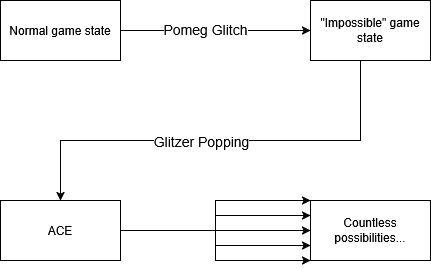
\includegraphics[width=0.5\textwidth]
		{figures/ace_img.png}}
	\caption{A scheme illustrating the process to achieve ACE}\label{fig:ace_scheme}
\end{figure}

The starting point for this chain is the \textit{Pomeg glitch} (chapter~\ref{sec:pomeg_glitch}), a glitch that allows the player to reduce a Pokémon’s HP below zero outside of battle, causing the game to enter an invalid state. When attempting to initiate a battle under these conditions, the game creates a placeholder Pokémon to avoid crashing, unknowingly opening the door to deeper exploitation. By examining this placeholder in battle, players can set up conditions to trigger another glitch known as \textit{Glitzer Popping} (chapter~\ref{sec:glitzer_popping}), which involves renaming the in-game PC storage boxes in a precise way. This process, along other steps, ultimately leads the game into treating the renamed data as if it were valid Pokémon data, and eventually as executable code.
This setup causes memory to be misread and reinterpreted and with careful planning, players can direct the game to areas of memory that contain useful data, or even custom payloads, by taking advantage of how the game processes corrupted or invalid Pokémon entries. While this avoids the need for external tools or hacking devices, rendering this types of manipulations doable on any type of legitimate hardware (like a Game Boy), the level of control granted is surprisingly deep, even able to altering game logic and spawning items or Pokémon at will.
This can become a serious issue, as, although technically impressive and often used only for speedrunning, this type of ACE could have lead to a monetary loss for the Pokémon Company. This is because, when the game originally came out in 2004, the company used to hold special in-person events where some rare Pokémon were given out to players (and this used to be the only way to get these Pokémon), as such, for anyone to be able to "generate" them through a couple of glitches it would make this a problem for the company, as the players would not need to attend this highly publicized events to get the Pokémon.


\subsection{The Pomeg glitch}
\label{sec:pomeg_glitch}
In Pokémon Emerald, the player can use a glitch called \textit{Pomeg glitch} to put the game in an impossible state. To explain this glitch first it would be wise to understand how the game roughly works. In Pokémon Emerald the player can be in two states: the exploration state, where they can go around the map with a team of up to six Pokémon, and the battle state, which is where the fighting happen. Any Pokémon caught after the sixth gets sent in the PC, which is a storage system that allows the player to store Pokémon that they do not want to carry with them. The Pokémon have their own statistics, which improve based on their levels and what other Pokémon they fight. The statistic involved with the Pomeg glitch is \textit{HP} (Hit Points), which is the amount of health a Pokémon has. If a Pokémon's HP reaches 0, it faints and cannot be used until it is revived plus, if all of them reach 0, we get a game over and this can only happen when the game is in the battle state.

The HP statistic is calculated through the following formula:

\begin{equation}
	\text{HP} = \left( \frac{(2 \times \text{Base} + \text{IV} + \left( \frac{\text{EV}}{4} \right)) \times \text{Level}}{100} \right) + \text{Level} + 10
	\label{eq:pokemon_hp_formula}
\end{equation}

This formula yields the maximum HP of a Pokémon, which is the maximum amount of health it can have. In the case of the \textit{Pomeg glitch}, the only relevant variable is the EV value: this is because the EV value is the only statistic that can be directly modified based on the actions of the player. It is an integer between 0 and 255, and it increases every time a Pokémon defeats another, but most importantly it can also be decreased by using certain items. In the case of the \textit{Pomeg glitch}, the player can use a specific item called \textit{Pomeg berry} (hence the name) to lower the EV value of a Pokémon by 10. However, if, for example, the Pokémon's current HP was at 1, when updating the newly calculated HP statistic, both the current HP and max HP get lowered and as such, the game could set the current HP value to 0, or, even worse, something below it, like underflowing to $ 2^{16}-1$ or 65535 HP (due to the HP statistic being an unsigned two-bytes integer). Now, to use a \textit{Pomeg berry} the player needs to not be in the combat state, and this can create some issues because the game is only capable of handling game overs (which happens when all of the player's Pokémon reach 0 HP) if the player is in a combat state. The problem arises in the situation where the Pokémon whose HP is being updated is the only one with $HP > 1$, because the player may end up with a party of only dead Pokémon, as can be seen in the figure below.

\begin{figure}[h!]
	\center{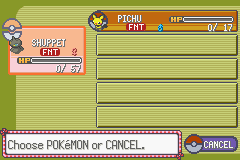
\includegraphics
		{figures/dead_team.png}}
	\caption{A technically impossible state}\label{fig:dead_team}
\end{figure}

This is not a problem right as it happens, however if the player is to start a battle, the game will try to look for a Pokémon to fight with, and it will find none, because all of them are dead. So after unsuccessfully looking for a Pokémon, the game will then send out a \textbf{?-like} Pokémon (commonly known in the Pokémon community as \textbf{Decamark})\footnote{https://bulbapedia.bulbagarden.net/wiki/Ten\_question\_marks} as can be seen in figure \ref{fig:decamark}, which is used to prevent game crashes, as when the game fails to load a proper Pokémon sprite, the Decamark is used as a placeholder.

\begin{figure}[h!]
	\center{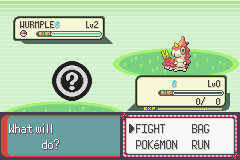
\includegraphics
		{figures/decamark.png}}
	\caption{The decamark Pokémon}\label{fig:decamark}
\end{figure}

At this point, the player can try to fight, run away or use an item, all options which would result in a white out (the game over mechanic). But how can this lead to ACE? This is where the glitch known as \textit{Glitzer Popping} comes into play.

\subsection{Glitzer Popping}
\label{sec:glitzer_popping}
The \textit{Pomeg data corruption glitch}, most commonly known as the \textit{Glitzer Popping}, is a glitch that allows the player to execute some arbitrary code by renaming the boxes to a specific string, which will then be interpreted as some ARM-Assembly code (since Pokémon Emerald is written in C and ARM-Assembly\footnote{https://pokemondb.net/pokebase/257153/what-programming-language-generations-series-games-written}) that will be executed when the game tries to read the name of the box. The player can rename the boxes in many different ways, obtaining different results spanning from obtaining event-exclusive items or Pokémon (for Pokémon Emerald many events were held in-person at some specific locations), to modify player information or game flags, all the way to being able to execute custom scripts (like creating your own events). "But how do we get the game to read the name of the box to the point where it gets executed?" is the most logical follow-up question. The answer is simple: we need to use the \textit{Pomeg glitch}.


\subsubsection{The setup}
\label{sec:setup}
First things first, this thesis is not a tutorial on how to achieve these glitches, as there are countless fantastic other guides about replicating them (like this video made by Youtuber PapaJefé\footnote{https://www.youtube.com/watch?v=45kwOEhKbUg}, or this guide made by Mickaël Laurent\footnote{https://e-sh4rk.github.io/ACE3/}), rather, my purpose is to illustrate and figure out why and how does ACE happen, using Pokémon Emerald as a basis for it.

To actually start executing some arbitrary code we need two things: the first one is the previously illustrated \textit{Pomeg glitch}, where the player is able to setup an impossible game state, and the second one needs the boxes in which the Pokémon that don't fit in the player's team are stored. These are 14 different boxes in which the Pokémon are stored, and they can be renamed by the player. The names of these boxes are stored in a specific area of the memory, and this is where \textit{Glitzer Popping} comes into play: as previously stated it is a technique that allows the player to execute some arbitrary code by renaming the boxes to a specific string, which will then be interpreted as some code that will be executed when the game tries to read the name of the box (an example can be seen in table \ref{tab:boxes_names}; \textbf{note}: in the game, the three dots are represented by a single character "\dots").

\begin{table}[h!]
	\centering
	\begin{tabular}{|c|l|}
		\hline
		\textbf{Box} & \textbf{Name}  \\
		\hline
		Box 1        & (VTTnFMBn)     \\
		Box 2        & (EEENJRo )     \\
		Box 3        & (EE5\dots q  ) \\
		Box 4        & (EFF\dots    ) \\
		Box 5        & (KT?nTR?n)     \\
		Box 6        & (EEEIP?n )     \\
		Box 7        & (EE'FQm  )     \\
		Box 8        & (EmFlo   )     \\
		Box 9        & (yLRom"Ro)     \\
		Box 10       & (EEEFGEn )     \\
		Box 11       & (EE \dots q  ) \\
		Box 12       & (E\dots -n   ) \\
		Box 13       & (FQRn\dots Rn) \\
		Box 14       & (EEEt ?n )     \\
		\hline
	\end{tabular}
	\caption{Example box names required to teleport to map ID \texttt{0B10}}
	\label{tab:boxes_names}
\end{table}


The game is not capable of handling the situation where the player has a Decamark in their team, and as such when the player tries to open their team information in battle it will unsuccessfully try to read the Pokémon's data from the memory, leaving instead a blank Pokémon.

So when the player moves the cursor to the first slot in their team, the cursor actually underflows and goes to slot 256 (since a team is made up of a maximum of 6 Pokémon) and as such, instead of scrolling through slots 1-6, the player has access to slots 255 and above (as the cursor is technically out of bounds). However, slots outside the first 6 aren't meant to be Pokémon slots, so the game accesses random blocks of RAM data and treats them as Pokémon, even though they are not. In this case the 255th party slot is actually the PC Pokémon data and continuing to scroll upwards allows the player to actually go over memory addresses reserved for various in-game data.

Each time the party Pokémon selection pointer moves to a new party slot, an anti-cheat verification routine is triggered for the selected "Pokémon" (because the game thinks it is one, but it's actually not). If the checksum of the selected data block (interpreted as a Pokémon) is invalid, the game modifies it into a Bad Egg, which is the result of the anti-cheating protocol. This transformation involves setting the Egg Status flag to 1 and enabling two additional bits, which designate the egg as a "Bad" Egg, whose in-game aspect can be seen in figure \ref{fig:bad_egg}. Since the memory blocks being interpreted as party Pokémon are not genuine Pokémon structures, their checksums will almost always be invalid unless the slot is empty, or accurately prepared.

\begin{figure}[h!]
	\center{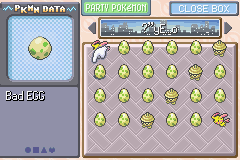
\includegraphics
		{figures/bad_egg.png}}
	\caption{A corrupted Pokémon that got labeled as a "Bad Egg"}\label{fig:bad_egg}
\end{figure}

\subsubsection{Pokémon data structure}
\label{sec:data_structure}
A Pokémon's data structure is made up of 100 bytes (which can be seen in table \ref{fig:full-pokemon-structure}), with many static (in the sense that once created they never get modified again) and some other dynamic fields (in the sense that they can be modified during the game). The static fields are used to store information about the Pokémon, such as its species, nickname, and trainer ID (TID, which is a 4-bytes (a double-word in C) long integer ranging from 0 to 65'535 that gets generated when the player starts the game for the first time), while the dynamic fields are used to store information about the Pokémon's current state, such as its level, experience points, current HP, etc.
The order of these information remains the same for every Pokémon except for the "Inner data" substructure (the substructure that starts at offset 0x20 in table \ref{fig:full-pokemon-structure}) which contains other generic information about the Pokémon: the structure is divided into four substructures, each of which is 12 bytes long. The first substructure contains the growth information, the second one contains the attacks, the third one contains the EVs and condition, and the last one contains miscellaneous information.

\begin{table}[h!]
	\centering
	\begin{tabular}{|c|c|c|}
		\hline
		\textbf{Name}          & \textbf{Offset (hex)} & \textbf{Length (bytes)} \\
		\hline
		Personality value      & 0x00                  & 4                       \\
		OT ID                  & 0x04                  & 4                       \\
		Nickname               & 0x08                  & 10                      \\
		Language               & 0x12                  & 1                       \\
		Misc. Flags            & 0x13                  & 1                       \\
		OT name                & 0x14                  & 7                       \\
		Markings               & 0x1B                  & 1                       \\
		Checksum               & 0x1C                  & 2                       \\
		Padding                & 0x1E                  & 2                       \\
		Inner data (encrypted) & 0x20                  & 48                      \\
		Status condition       & 0x50                  & 4                       \\
		Level                  & 0x54                  & 1                       \\
		Mail ID                & 0x55                  & 1                       \\
		Current HP             & 0x56                  & 2                       \\
		Total HP               & 0x58                  & 2                       \\
		Attack                 & 0x5A                  & 2                       \\
		Defense                & 0x5C                  & 2                       \\
		Speed                  & 0x5E                  & 2                       \\
		Sp. Attack             & 0x60                  & 2                       \\
		Sp. Defense            & 0x62                  & 2                       \\
		\hline
	\end{tabular}
	\caption{Full Pokémon Data Structure (Generation III)}
	\label{fig:full-pokemon-structure}
\end{table}

This substructure is the most relevant for a Pokémon as it contains the most important information about the Pokémon itself, on top of being key to verify a Pokémon's data integrity. How that part is handled is that the order of these four substructures is determined by the Pokémon's Personality Value (PID, which is an 8-bytes long integer that gets generated when a Pokémon's data is first created) and the TID. The formula used to determine the order of the substructures is as follows:

\begin{equation}
	\left( \texttt{TID} \oplus \texttt{PID} \right) \bmod 24
	\label{eq:substructure_order_formula}
\end{equation}

The game takes the TID and the PID, lengthens the TID to the length of the PID by adding 0s to it and XORs it with the PID, and then takes the result modulo 24. The result of this calculation is then mapped directly to the substructure order table (table \ref{tab:substructure-order}) to determine the order of the substructures, where G stands for the growth substructure, A stands for the attacks one, E is the EVs and condition one and M is the miscellaneous substructure.

\begin{table}[h!]
	\centering
	\begin{tabular}{cccc}
		\toprule
		00. GAEM & 06. AGEM & 12. EGAM & 18. MGAE \\
		01. GAME & 07. AGME & 13. EGMA & 19. MGEA \\
		02. GEAM & 08. AEGM & 14. EAGM & 20. MAGE \\
		03. GEMA & 09. AEMG & 15. EAMG & 21. MAEG \\
		04. GMAE & 10. AMGE & 16. EMGA & 22. MEGA \\
		05. GMEA & 11. AMEG & 17. EMAG & 23. MEAG \\
		\bottomrule
	\end{tabular}
	\caption{Substructure order based on PID\%24}
	\label{tab:substructure-order}
\end{table}


Because these substructures are encoded using the Pokémon’s PID and the Trainer ID (TID), setting the Egg Status flag to 1 can result in either a bit value of 1 or 0, depending on the result of \texttt{PID} XOR \texttt{TID}. Out of all of the different locations within a Pokémon's data structure, the Egg Status flag resides in the miscellaneous slot, however, in contrast, the two bits that define a "Bad" Egg are always located at fixed positions at offset 0x13 of the Pokémon's data in the "Misc. flags" slot, and they are consistently set to 1 when a checksum is invalid.

\begin{table}
	\begin{center}
		\begin{tabular}{|c|c||c|c||c|c||c|c|}
			\hline
			\multicolumn{2}{|c||}{\textbf{Growth}}          &
			\multicolumn{2}{c||}{\textbf{Attacks}}          &
			\multicolumn{2}{c||}{\textbf{EVs \& Condition}} &
			\multicolumn{2}{c|}{\textbf{Miscellaneous}}                                                                              \\
			\hline
			\textbf{Name}                                   & \textbf{Bytes} &
			\textbf{Name}                                   & \textbf{Bytes} &
			\textbf{Name}                                   & \textbf{Bytes} &
			\textbf{Name}                                   & \textbf{Bytes}                                                         \\
			\hline
			Species                                         & 2              & Move 1 & 2 & HP EV      & 1 & Pokérus status      & 1 \\
			Item held                                       & 2              & Move 2 & 2 & Attack EV  & 1 & Met location        & 1 \\
			Experience                                      & 4              & Move 3 & 2 & Defense EV & 1 & Origins info        & 2 \\
			PP bonuses                                      & 1              & Move 4 & 2 & Speed EV   & 1 & IVs, Egg, Ability   & 4 \\
			Friendship                                      & 1              & PP 1   & 1 & Sp. Atk EV & 1 & Ribbons + Obedience & 4 \\
			Unused                                          & 2              & PP 2   & 1 & Sp. Def EV & 1 &                     &   \\
			                                                &                & PP 3   & 1 & Coolness   & 1 &                     &   \\
			                                                &                & PP 4   & 1 & Beauty     & 1 &                     &   \\
			                                                &                &        &   & Cuteness   & 1 &                     &   \\
			                                                &                &        &   & Smartness  & 1 &                     &   \\
			                                                &                &        &   & Toughness  & 1 &                     &   \\
			                                                &                &        &   & Feel       & 1 &                     &   \\
			\hline
		\end{tabular}
		\caption{Pokémon data structure by substructure (12-bytes blocks)}
		\label{table:pokemon-data-structure}
	\end{center}
\end{table}

\newpage

An additional layer of randomness is introduced by the DMA (Direct Memory Access) system, which is another built-in anti-cheat mechanism that shifts the RAM addresses of numerous data structures whenever the player performs actions such as entering a battle, going through a doorway, or opening the in-game bag. The DMA remaps memory addresses using a translation table of multiple double-words. Any value subjected to DMA can occupy up to 32 different memory addresses, each spaced by 4 bytes.

Importantly, party Pokémon are not affected by DMA, which means the memory addresses of the six standard party slots remain fixed. However, any data read from memory locations beyond the sixth slot \textit{is} subject to DMA. Since each party Pokémon occupies 25 double-words, and DMA remapping allows up to 32 double-word shifts, each double-word in a slot beyond the sixth could potentially be placed at an address susceptible to corruption via the Egg Status bit alterations. Due to the variability in both RAM content and corruption locations, these elements may interact unpredictably, sometimes preventing a given double-word from being corrupted by the Egg-related flags.

Through the use of carefully planned strategies (like the \textit{Glitzer Popping}), it becomes possible to intentionally corrupt specific values within the data of a Pokémon, while simultaneously ensuring that surrounding data remains unaffected, thus enabling a form of highly targeted or pinpoint corruption. This capability allows for the precise manipulation of a Pokémon's PID and/or TID within the PC storage system, without altering the remainder of the Pokémon’s structured data. Since both the PID and TID serve a crucial role in encrypting Pokémon’s four internal substructures, with each one containing different categories of the Pokémon’s information, the corruption of these values causes a dramatic shift in the Pokémon’s checksum, which functions as a form of data integrity verification.

Among the known corruption methods, the two specific bits responsible for creating so-called "Bad Eggs" are not suitable for intentional and controlled Pokémon data corruption, as they invariably fail to preserve the checksum, rendering the resulting data unstable and largely unusable. In contrast, a more nuanced method (corruption via the Egg State Flag) offers a much more promising avenue, as it allows for manipulation while keeping the checksum intact. This method alters the checksum by a multiple of 0x4000, and because the checksum is stored as a 16-bit word, any change that corresponds to an even multiple leaves the checksum effectively unchanged. Although there exist certain rare conditions under which this multiple might be odd, thus compromising the checksum, these conditions can be easily identified and prevented, allowing for a consistently reliable corruption method that keeps the data within safe bounds.

Since the PID governs the order in which the four data substructures are stored and subsequently read by the game, corrupting it directly alters this order, resulting in the game interpreting one category of data as another: for example, reading what is meant to be the Moves substructure as if it were the EVs substructure. This misinterpretation of substructure order becomes a powerful tool for altering multiple facets of a Pokémon's attributes such as its species, held item, experience points, individual values (IVs), effort values (EVs), friendship level, obedience flag, origin data, and of course, its moveset, simply by assigning specific values to those fields prior to the corruption process. Although there are theoretically 24 different ways to reorder the four substructures, only 10 permutations are actually possible within the game’s mechanics when doing a corruption. These ten permutations are collectively referred to as Corruption Types, and each one produces unique effects based on how the substructure data is reorganized, meaning that the specific impact of a PID corruption is entirely determined by which Corruption Type is applied.

However, even when using the Egg State Flag corruption technique, which successfully preserves the Pokémon’s checksum and alters the substructure order as intended, the change to the encryption key (caused by modifying either the PID or TID) can still introduce undesirable side effects. These side effects include transforming the Pokémon into an Egg, assigning glitched or unusable moves to the second and fourth move slots, or disrupting other internal values that affect gameplay. The presence of a corrupted Pokémon in an Egg state poses a significant drawback, as the act of hatching resets many of its attributes and, in the case of certain Glitch Pokémon, can result in game crashes or freezing. Furthermore, corrupted move slots can restrict the player from using, viewing, reordering, or replacing the affected moves, thus limiting the Pokémon's functionality and strategic use.

To mitigate these problems and produce a clean, stable result, an advanced technique involves performing two successive \textit{Glitzer Popping} procedures, first corrupting the PID, and then the TID (or vice versa) in a way that ensures the Pokémon ends up with a valid checksum, a desired change in substructure order, and, importantly, a restoration of its original encryption key through the reversal of the PID or TID alteration. This dual-step approach ensures that the corrupted Pokémon retains its intended modifications while eliminating residual glitched values, effectively enabling the precise and consistent corruption of nearly any Pokémon without the drawbacks typically associated with such manipulations.


\subsubsection{Running the code}
\label{sec:running_the_code}
Through the aforementioned glitches, it's possible to create a corrupted Pokémon that, when hatched, due to the stable corruption will have some of its data switched: due to the corruption of the PID and the TID, now the result of equation \ref{eq:substructure_order_formula} will be different, and as such the order of the substructures will be different, but it will maintain the previous values. For example a Pokémon whose checksum gave it an order of GAEM could (since the corruption has some casualty to it due to DMA) end up being ordered as EAGM, which means that the game will read the data in a different order than it was originally intended and if the HP EV value was 0x06 (6 in decimal) while the Attack EV value was 0x11 (17 in decimal), the game will now read the Species value as 0x0611 (since the Species value uses 2 bytes and the HP and Attack EVs only use 1) and vice-versa (this process can be seen visualised in figure \ref{fig:corruption_substructures}). This, as previously mentioned, creates a problem when trying to reference the Pokémon's sprite animation, as the address of one's sprite animation is directly based on its species value.

\begin{figure}[h!]
	\center{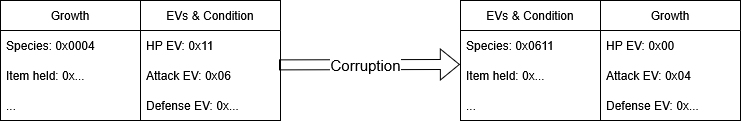
\includegraphics[width=0.85\textwidth]
		{figures/corruption_substructures.png}}
	\caption{Visual representation of the corruption of the substructures}
	\label{fig:corruption_substructures}
\end{figure}

Therefore, when a Pokémon egg hatches, the animation gets played (as shown in figure \ref{fig:sprite_animation}), and the game will then try to read the Pokémon data from the memory, however the address is not the one of a valid animation since in Pokémon Emerald only IDs of up to 0x0183 are occupied by actual animations.

\begin{figure}[!htb]
	\centering
	\subfloat[First frame]{
		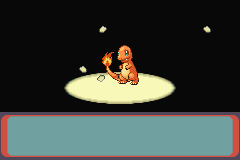
\includegraphics[width=0.25\textwidth]{figures/charmander_hatch.png}}
	\label{fig:First frame of the hatching animation}
	\qquad
	\subfloat[Second frame]{
		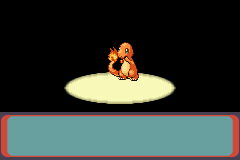
\includegraphics[width=0.25\textwidth]{figures/char_animation.png}}
	\label{fig:Second frame of the hatching animation}
	\qquad
	\subfloat[Final frame]{
		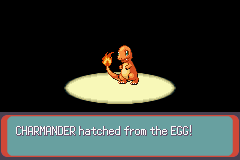
\includegraphics[width=0.25\textwidth]{figures/char_end_animation.png}}
	\label{fig:Final frame of the hatching animation}
	\caption{Sprite animations}
	\label{fig:sprite_animation}
\end{figure}


As seen in table \ref{tab:boxes_names_explanation}, the code that gets executed ultimately ends up actually being a series of ARM Assembly instructions, which are then executed by the game. And this is ultimately where ACE happens: since ARM Assembly is a low-level programming language, if the species ID points to a "wrong" or "unintended" entity, instead of crashing, it just reads and executes what is found there. In our example the table for the animations has valid entries up to 0x50, but since the function that handles this is capable of reading up to 0xFF, and entry 0x6e is where the PC boxes names start, the game erroneously reads and executes the PC box names.



\section{Detecting and Preventing Arbitrary Code Execution}
\label{sec:state_of_the_art}

In chapter \ref{sec:case_study} we have seen how ACE can be achieved through the use of glitches in Pokémon Emerald, and how it is possible to execute some arbitrary code. In figure \ref{fig:ace_scheme} we saw how ACE is achievable through the chaining of glitches, and the first one of these, the \textit{Pomeg glitch}, is born out of a simple missing if statement that doesn't check if the Pokémon's HP is greater than 1 before trying to use the berry. This is a simple mistake that can be easily fixed nowadays, either through updates or patches, but in 2004 when the game originally released this was not possible. In this chapter we will see how ACE can be detected and prevented in modern systems, and we will be looking at the current state of the art in the field of ACE detection and prevention by analysing much recent scenarios and papers.

Initially, in chapter \ref{sec:today}, the focus will be on detection, and the article we will be looking at is \textit{"Detection of Remote Code Execution vulnerability in website source codes using LSTM machine learning model"}\footnote{https://www.researchgate.net/publication/381650864\_Detection\_of\_Remote\_Code\_Execution\_vulnerability\_in\_website\_source\_codes\_using\_LSTM\_machine\_learning\_model} by Armin Zakarian and Muhammad Rahmani, which was published in 2024. The paper focuses on the detection of Remote Code Execution (RCE) vulnerabilities in web applications, which is a type of ACE that can be exploited by attackers to execute arbitrary code on a target system.

The authors propose a machine learning-based approach to detect RCE vulnerabilities in web application source codes, using Long Short-Term Memory (LSTM) networks to analyze the source code and identify potential vulnerabilities.
After which, the focus, in chapter \ref{sec:current_studies}, will be on prevention, and the articles we will be looking at are: \textit{"EC-CFI: Control-Flow Integrity via Code Encryption Counteracting Fault Attacks"}\footnote{https://arxiv.org/abs/2301.13760} which was published in 2023 by Pascal Nashal, Salmin Sultana, Hans Liljestrand et al. plus \textit{"G-Free: defeating return-oriented programming through gadget-less binaries"} published in 2010 by Kaan Onarlioglu, Leyla Bilge, Andrea Lanzi, Davide Balzarotti, et al. The papers focus on the prevention of ACE vulnerabilities in embedded systems, which are often targeted by attackers due to their limited resources and lack of security measures.


\subsection{Detection}
\label{sec:today}

As illustrated in chapter \ref{sec:ace}, ACE and the detection of its vulnerabilities remains a critical challenge in contemporary web application security. In this context, the study titled \textit{"Detection of Remote Code Execution vulnerability in website source codes using LSTM machine learning model"} proposes a novel detection framework leveraging LSTM networks to identify potential RCE threats, which are a subset of ACE vulnerabilities; the difference, albeit simple, is that RCE does not require the attacker to have prior access to the system, plus they exploit a different type of vulnerability. While ACE generally exploits software bugs and/or memory corruption, RCE uses APIs or web-apps, hence why the name \textbf{Remote} Code Execution. Traditional detection mechanisms, such as static code analysis or signature-based scanning, often fall short when dealing with obfuscated or dynamically generated exploit patterns. The LSTM-based model introduced in the paper addresses this limitation by learning semantic and syntactic dependencies in source code sequences. Specifically, the system is trained on a labeled dataset containing both benign and malicious PHP code samples, enabling it to classify code fragments with high accuracy based on their learned contextual features. The model architecture benefits from the LSTM's ability to retain long-term dependencies, making it particularly suited for recognizing exploit patterns that may be distributed across multiple lines or functions. The authors report promising accuracy and precision metrics, suggesting the model's practical applicability in real-world detection pipelines. Moreover, the system does not rely heavily on handcrafted features, making it adaptable to different codebases and scalable to larger projects. This approach exemplifies the growing role of deep learning in static code analysis and demonstrates a feasible path toward automating RCE detection in web application environments.

\subsubsection{LSTM-Based Detection Approach}
The detection framework suggested by Zakarian and Rahmani utilizes LSTM networks to identify RCE vulnerabilities in source code, specifically within PHP-based web applications. LSTM networks are a specialized type of recurrent neural network (RNN) designed to model and learn from sequential data where long-range dependencies are important. Unlike standard RNNs, which suffer from vanishing or exploding gradients (which are, respectively, when a gradient becomes either too small to update weights effectively, or when it becomes excessively large to the point of destabilizing it) during backpropagation through time (BPTT), LSTMs incorporate a series of gates, specifically: input, forget, and output gates, that control the flow of information into and out of a cell state, effectively allowing the network to retain or discard information across time steps. This gating mechanism enables LSTMs to maintain relevant contextual information over long sequences, making them particularly well-suited for tasks such as natural language processing, speech recognition, and increasingly, source code analysis. In the context of vulnerability detection, LSTMs can capture the relationships between syntactic tokens and control structures scattered across different parts of a program, learning patterns that may indicate the presence of insecure or exploitable code.

In their implementation, the authors prepare a labeled dataset consisting of source code snippets classified as either vulnerable or non-vulnerable with respect to RCE exploits. Vulnerable examples typically contain known exploit patterns, such as the use of \textit{eval}, \textit{system}, or \textit{shell\_exec} functions in contexts where user-controlled input is insufficiently sanitized. To then make the code suitable for learning, a pre-processing pipeline is applied, which involves lexical tokenization (breaking code into syntactic units), normalization (abstracting variable names, constants, and function arguments), and transformation into fixed-length sequences, which are then vectorized before being fed into the LSTM network.

The model architecture typically includes one or more layers of LSTM units followed by fully connected layers that produce a binary output, indicating whether a given snippet is likely to contain a vulnerability. The output is interpreted as a probability score, and a threshold is applied to classify the input as vulnerable or safe. During training, the model is presented with many examples from the labeled dataset and adjusts its internal parameters to minimize the difference between its predictions and the actual labels. This is done using a standard optimization process, which involves calculating errors and adjusting the network’s weights accordingly over many iterations to avoid a vanishing or exploding gradient.

Once trained, the model can be evaluated using common performance metrics such as precision (how many detected vulnerabilities are actually real), recall (how many real vulnerabilities the model manages to find), and F1-score (a balanced measure that considers both precision and recall). According to the results presented by Zakarian and Rahmani, the LSTM-based model demonstrated strong performance, successfully identifying vulnerable code patterns even in cases where the exact syntax or structure varied from the training data.

According to the authors, what makes this approach particularly promising is its flexibility: unlike rule-based systems that rely on predefined patterns and are easily bypassed by code obfuscation or slight rewrites, the LSTM model learns the underlying relationships in code that are commonly associated with insecure practices. This allows it to generalize better and potentially detect novel or unexpected vulnerability patterns. While not without limitations (such as the need for large, high-quality training data and relatively high computational cost) the approach represents a significant advancement in automated vulnerability detection and opens the door to broader applications in software security.

\subsubsection{Implications, Limitations and Possible Extensions}

The LSTM-based detection approach presented by Zakarian and Rahmani offers a number of practical and conceptual implications for the broader field of software vulnerability analysis and most notably, it illustrates the effectiveness of applying sequence models to source code, treating code not simply as static syntax but as a structured, time-aware data stream where context and order matter significantly. This shift—from rule-driven scanning to context-aware learning—represents an important step forward in detecting vulnerabilities that are subtle, context-dependent, or deliberately obfuscated which often are not given enough importance, due to a lack of resources (may it be money, time, or both). For developers and security analysts, this kind of tool could be integrated into development environments or CI/CD pipelines to automatically flag suspicious code as it is written or deployed, offering real-time feedback and reducing the risk of RCE vulnerabilities reaching production.

That said, there are also important limitations to consider. One of the most immediate is the dependency on a well-labeled and representative dataset. In the original study, the model was trained exclusively on PHP code, which means its performance on other languages or frameworks is uncertain without retraining. Each language has its own syntax and security risks, and a model trained on one may not generalize to another without careful adaptation. In addition, while LSTMs are capable of capturing long-term dependencies, they are still not inherently interpretable; the model may flag a piece of code as dangerous, but without offering a clear explanation, which can reduce trust and make it harder for developers to take corrective action. Techniques such as attention mechanisms or post-hoc explainability tools could potentially be used to improve transparency, but these were not explored in the referenced study.

From a computational standpoint, training deep learning models such as LSTMs is resource-intensive, requiring both time and hardware (typically GPUs) to process large datasets effectively. While prediction, once trained, is relatively fast, the training phase presents a barrier to entry for smaller teams or projects without dedicated machine learning infrastructure. Furthermore, the model’s effectiveness is tied to the quality of its training data; if the dataset is outdated or biased toward certain types of vulnerabilities, the model may fail to detect new or less common exploit patterns.

Despite these challenges, the approach has considerable potential for extension, especially with the advancements in the machine learning fields of the last years. With sufficient data and adjustments to preprocessing, the model could be adapted to other programming languages or application domains. For example: the same principles could be applied to smart contracts, embedded firmware, or interpreted game scripts, where code is similarly structured and context-sensitive. In the context of this thesis, which explores ACE in environments outside traditional web applications, the success of the LSTM model in learning RCE patterns suggests that machine learning could likewise be applied to detect or even prevent ACE in unconventional domains, given a suitable representation of the code or memory structure.

Ultimately, while still in early stages compared to traditional static analysis tools, the use of LSTM networks for vulnerability detection represents a promising evolution in security automation. With a (possibly) growing interest on the topic and refinement of its techniques, such models could become a foundational component of future secure development practices.

\subsection{Prevention}
\label{sec:current_studies}

% EC-CFI: Control-Flow Integrity via Code Encryption Counteracting Fault Attacks
Preventing ACE requires robust mechanisms that can enforce strict control over a program’s execution flow, especially in the presence of fault injection and memory corruption attacks. The paper titled \textit{"EC-CFI: Control-Flow Integrity via Code Encryption Counteracting Fault Attacks"} introduces a cryptographically enforced Control-Flow Integrity (CFI) scheme designed to counteract such threats at runtime. EC-CFI operates by encrypting code blocks and tightly coupling decryption with legitimate control-flow transitions, ensuring that only authorized instruction sequences can be executed. This method effectively blocks attempts to divert execution toward malicious or unintended code paths, which are characteristic of ACE exploits. The authors present a hardware-software co-design that allows encrypted instructions to be decrypted on-the-fly only when control transfers are validated against a predefined control-flow graph. Any unauthorized deviation results in execution failure, thereby neutralizing potential exploit vectors. The proposed technique is particularly effective against fault injection attacks, which aim to manipulate program behavior by corrupting control data. Experimental results demonstrate that EC-CFI offers strong security guarantees with modest performance overhead, making it suitable for deployment in resource-constrained environments such as embedded systems and IoT devices. By employing code encryption as a runtime enforcement mechanism rather than relying solely on static checks, EC-CFI presents a proactive and resilient approach to mitigating ACE risks. This work exemplifies a shift toward stronger, cryptographically-backed security primitives in control-flow enforcement, positioning itself as a forward-looking solution for future system architectures.

% G-Free: defeating return-oriented programming through gadget-less binaries
ACE vulnerabilities, particularly those exploited through Return-Oriented Programming (ROP) techniques, pose significant threats to software security. ROP is a specific exploitation method used to achieve ACE by chaining together small instruction sequences already present in a program’s memory, typically using return instructions to control flow; while ACE is the end goal, ROP is one of the strategies used to reach that goal, especially in environments protected against traditional code injection techniques like those that use Data Execution Prevention (DEP, a security feature that prevents code from being executed in certain regions of memory that are intended only for data). The paper titled \textit{"G-Free: Defeating Return-Oriented Programming through Gadget-less Binaries"} introduces a compiler-based approach designed to mitigate such threats by eliminating exploitable code sequences, known as "gadgets," from binary executables. G-Free operates by identifying and removing unaligned free-branch instructions, such as unintended \texttt{ret} instructions that may arise due to instruction alignment, and by protecting aligned free-branch instructions through encryption mechanisms. Specifically, G-Free modifies the compiler backend to ensure that return addresses are encrypted upon function entry and decrypted before function return, thereby preventing attackers from manipulating return addresses to redirect control flow maliciously. This approach effectively neutralizes the primary mechanism by which ROP attacks chain together existing code snippets to perform unauthorized operations. The authors implemented G-Free as a prototype within the GNU Compiler Collection (GCC) and evaluated its effectiveness by compiling and testing real-world applications, including the GNU C Library (glibc). The results demonstrated that G-Free successfully eliminated usable gadgets without requiring source code modifications or additional runtime support, incurring an average performance overhead of only approximately 3\%. By proactively restructuring binaries to be "gadget-less," G-Free offers a practical and efficient defense against ACE vulnerabilities exploited through ROP, enhancing the overall security posture of compiled applications.

\subsubsection{G-Free: Compiler-Based Mitigation of Return-Oriented Programming}

%ROP Attacks and the motivation for G-Free

ROP is a sophisticated exploitation technique that emerged as a response to the growing adoption of runtime protections such as DEP, which enforces the separation between executable and writable memory, preventing attackers from injecting and running shell code directly. However, attackers adapted by reusing fragments of code that already exist in the binary, commonly referred to as gadgets, which typically end with a return instruction. By chaining these gadgets together, an attacker can construct arbitrary behavior without injecting new code, effectively bypassing DEP.

ROP exploits rely on the ability to manipulate the call stack so that the return address of a function is replaced with the address of a chosen gadget: by carefully constructing the stack, the attacker can direct execution through a sequence of return addresses, each pointing to a short code snippet ending in a return. These chains can mimic complex logic and even perform system-level operations, all while remaining within the bounds of executable memory, a principle demonstrated in practice by ACE exploits targeting, for example, Pokémon Emerald, as seen in chapter \ref{sec:case_study} (see figure~\ref{fig:rop}).

\begin{figure}[h!]
	\center{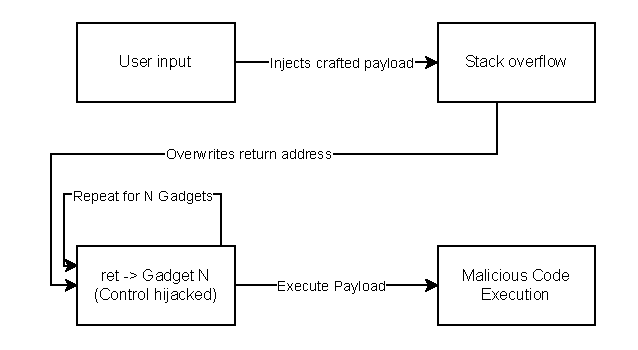
\includegraphics[scale=1]
		{figures/ROP.pdf}}
	\caption{A graphical illustration of a ROP attack\label{fig:rop}}
\end{figure}

This form of attack proved difficult to prevent using traditional countermeasures such as Address Space Layout Randomization (ASLR)\footnote{https://devblogs.microsoft.com/oldnewthing/20241024-00/?p=110417} or stack canaries alone. ASLR introduces variability into the memory layout, but on systems with limited entropy or known offsets, attackers can still reliably guess addresses. Stack canaries, while effective against simple buffer overflows, do not protect against control flow manipulation that does not overwrite the function's return path directly. As a result, a more comprehensive defense was needed, one that would directly address the mechanics of gadget-based exploitation.

G-Free was introduced in response to this need: it addresses ROP by modifying the binary during compilation to eliminate or neutralize the elements required to construct a successful ROP chain. Rather than detecting ROP attacks at runtime, G-Free prevents them proactively by ensuring that the compiled binary contains no usable return-oriented gadgets, as such its defense strategy operates on two main fronts: gadget elimination and return address protection (RAP), both implemented as part of the compilation process.

The first component, gadget elimination, involves scanning the binary for instruction sequences that can be misused as gadgets; these typically include short sequences of instructions ending with a ret (return) instruction, often occurring unintentionally in the middle of legitimate code due to instruction alignment or padding. G-Free modifies these potential gadgets by either restructuring them to remove exploitable patterns or inserting invalid instructions to break them. In doing so, it aims to make the binary “gadget-free,” at least in the context of chains that could be useful to an attacker.

The second component, RAP, involves encrypting return instructions so that they cannot be executed unless the control flow follows a legitimate call-return structure. During compilation G-Free inserts a unique cookie before each return address pushed to the stack during a function call and before returning this cookie is validated and removed. If an attacker attempts to hijack the control flow by inserting a fake return address, the absence or corruption of the cookie causes the program to crash or terminate. This mechanism ensures that return instructions can only be executed in the expected order, directly following a matching function call (see figure~\ref{fig:rop_protected}).

\begin{figure}[h!]
	\centering
	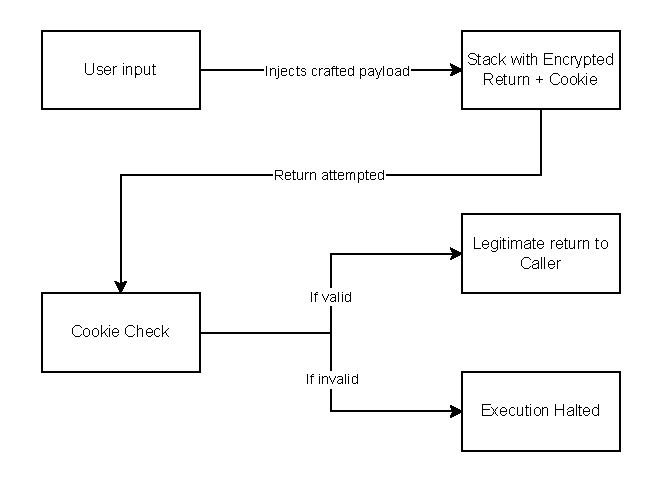
\includegraphics[scale=1]{figures/ROP-Protected.pdf}
	\caption{G-Free-enforced control flow}
	\label{fig:rop_protected}
\end{figure}

This design maintains compatibility with existing calling conventions while strengthening the integrity of control flow transitions. Because G-Free’s transformations occur at compile time, there is no need for additional runtime monitoring or kernel support, which makes the technique relatively lightweight from a systems perspective. However, this static nature also introduces constraints: the approach assumes that the binary remains unchanged post-compilation and that no dynamically generated or injected code will be executed at runtime. Additionally, any hand-written assembly or binary manipulation performed after compilation may invalidate G-Free’s guarantees.

The strength of G-Free lies in its simplicity and integration into the compiler toolchain, as it does not require hardware support or runtime instrumentation and it produces hardened binaries that are resistant to a broad class of code reuse attacks. While it may not provide complete security against every form of control-flow manipulation, it significantly raises the bar for attackers by eliminating the basic building blocks required for ROP. However, while G-Free is effective in reducing the number of usable gadgets and enforcing return integrity with minimal runtime cost, its static design limits its applicability to systems where full control over the compilation process is available. It does not address newer code-reuse techniques such as Jump or Call Oriented Programming (JOC and COP), and may be bypassed in environments where dynamic code generation or binary patching is present. Nonetheless, it represents an important step in compiler-based security and forms a conceptual basis for more advanced runtime defenses like EC-CFI.


\subsubsection{EC-CFI: Cryptographic Runtime Enforcement}

%Fault Injection and Control-Flow Attacks

As attackers adapted to static hardening techniques such as G-Free, more sophisticated control flow attacks began to emerge, including JOP and COP. These techniques avoided return instructions entirely by chaining together code sequences ending in indirect jumps or calls and since G-Free focused exclusively on protecting returns, it left other forms of indirect control transfers unguarded, exposing a broader surface for code reuse attacks. This class of attack shares structural similarities with return-oriented programming, shown previously in figure~\ref{fig:rop}, though it relies on call and jump instructions rather than returns. In response, the security community began to explore more comprehensive solutions, grouped under the broader category of control flow integrity.

Control flow integrity aims to prevent control hijacking by restricting indirect transfers, such as calls, jumps, or returns, to a predefined set of valid destinations extracted from the program’s control flow graph. While the conceptual model is sound, early implementations were often too permissive, allowing transfers to any function with a matching type signature or a compatible structure. This left space for attackers to build functional gadget chains even within the allowed target set, and other proposals required hardware features, runtime instrumentation, or significant compiler support, making them impractical or costly to adopt in real systems.

EC-CFI was introduced as an evolution of these earlier ideas, with the goal of enforcing precise, efficient, and complete control flow integrity across all indirect branches in real-world software. It modifies the binary at compile time by inserting metadata and validation logic that collectively verify whether a control transfer is legitimate. Each transfer site is analyzed statically to determine the exact set of allowed destinations, and these are grouped into equivalence classes based on shared behavior. Each class receives a unique identifier, and indirect branches are instrumented to verify that their targets belong to the appropriate class. If the check fails, execution halts, preventing unintended redirection of control flow (see figure~\ref{fig:ec_cfi_flow}).

\begin{figure}[h!]
	\centering
	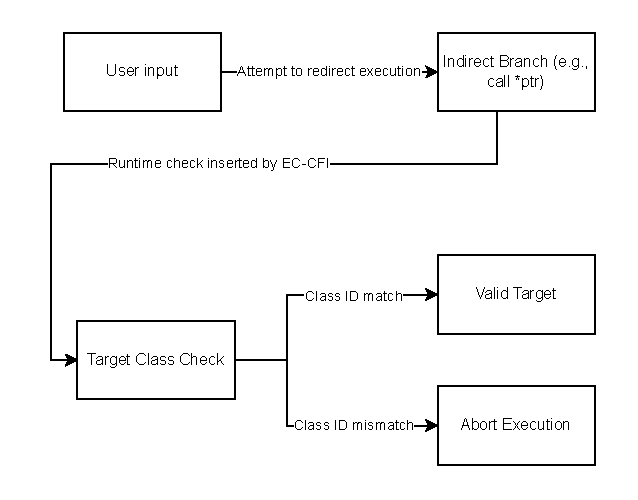
\includegraphics[scale=1]{figures/EC-CFI.pdf}
	\caption{EC-CFI validation step before each indirect control transfer}
	\label{fig:ec_cfi_flow}
\end{figure}


This approach allows EC-CFI to impose strict constraints on indirect transfers without introducing excessive performance overhead, since the validation relies on embedded metadata and avoids expensive runtime lookups, it achieves a balance between security and efficiency. Unlike previous systems that permitted control to flow to loosely defined sets of valid targets, EC-CFI restricts execution to the minimal set required for correct behavior, as determined through static analysis and therefore the result is a defense that blocks not only return-based reuse, but also attacks based on function pointers, virtual calls, and computed jumps.

Despite these improvements, EC-CFI is not without limitations. Its effectiveness depends heavily on the completeness and accuracy of the control flow graph extracted during compilation. If this graph fails to account for valid program behavior, the resulting checks may be overly restrictive, leading to false positives or program crashes. On the other hand, if the analysis is too permissive, it may admit unintended control flows. Like G-Free, EC-CFI assumes that the binary remains unchanged after compilation, and its guarantees may be invalidated by dynamic code generation, binary patching, or self-modifying code. In addition, the system requires full control over the build process, which limits deployment to environments where source code and compiler integration are available.

Even with these constraints, EC-CFI represents a substantial step forward in control flow security, as it generalizes the enforcement of structural integrity across the full range of indirect branches, closing gaps left by previous protections. By doing so, it offers a practical and broadly applicable method for defending against advanced control flow attacks in modern software systems.

%The EC-CFI Model

%Security Evaluation and Overhead

\subsubsection{Comparative Analysis of G-Free and EC-CFI}

G-Free and EC-CFI represent two distinct approaches to control flow protection, both grounded in compiler-level transformations but differing significantly in scope, complexity, and enforcement strategy. This is however expected, as one is a paper from 2010 (\textit{G-Free}) while the other is from 2023 (\textit{EC-CFI}). While G-Free focuses narrowly on securing return instructions to prevent return-oriented programming, EC-CFI expands the enforcement boundary to cover all forms of indirect control transfers. This distinction reflects a broader evolution in software security: from targeted mitigations aimed at specific exploit classes to comprehensive frameworks designed to defend against a wider variety of code reuse attacks.

The most immediate difference lies in the type of control transfers each system protects. G-Free operates specifically on return instructions by encrypting return addresses and eliminating gadgets that end in a return. It offers strong protection against attacks that rely on chaining such gadgets, but does not address indirect calls or jumps, which are commonly used in more advanced exploitation techniques such as jump-oriented or call-oriented programming. EC-CFI, on the other hand, provides a unified mechanism for validating all indirect branches, including returns, thereby offering broader coverage across the entire control flow surface of a program.

The enforcement mechanisms also differ in how they constrain behavior. G-Free uses a combination of static gadget removal and runtime cookie verification, which is relatively lightweight and requires minimal runtime overhead. EC-CFI relies on compile-time analysis to generate control flow metadata and injects runtime checks that validate each indirect transfer against its expected destination class. While EC-CFI introduces more instrumentation, its grouping of transfer sites with identical target sets ensures that the performance impact remains low in practice. In exchange, it achieves a much higher level of precision in allowed control flows.

From a deployment perspective, both systems require access to source code and the ability to instrument the binary during compilation. G-Free’s simpler model may make it easier to integrate in constrained or legacy environments, especially those where return-oriented programming is the primary concern. EC-CFI, while more complex, offers stronger and more general protections but assumes a more complete and accurate control flow graph, and may require careful tuning or additional annotations in codebases with indirect function dispatch or dynamic behaviors.

Security-wise, G-Free is effective in reducing the risk of traditional ROP attacks but is blind to attacks that operate through alternative control paths. EC-CFI closes this gap by enforcing structural correctness on all indirect branches, making it resilient against a wider class of modern exploits. However, EC-CFI’s strength depends on the accuracy of its static analysis. Incomplete or overly permissive graphs may introduce false positives or leave certain vulnerabilities exposed.

In summary, G-Free and EC-CFI should not be seen as competing solutions, but rather as part of a progression. G-Free laid the groundwork for compiler-based return protection, introducing the idea of proactively eliminating gadget-based attacks. EC-CFI extends this philosophy, generalizing it to provide full-spectrum protection across all indirect transfers.

\subsubsection{Integration with Detection Approaches}

While control flow integrity mechanisms such as G-Free and EC-CFI aim to prevent exploitation by enforcing valid control transfers at runtime, they do not analyze the semantics or intent of the source code itself. Their effectiveness lies in ensuring that control flow follows pre-defined, legitimate paths, but they operate at the binary level and only after the code has been compiled. As such, they do not address whether the code is safe or vulnerable in its logic or data handling.

In contrast, detection-based approaches (such as the LSTM-based model discussed in chapter \ref{sec:today}), operate earlier in the software development lifecycle. These models analyze raw or pre-processed source code to identify patterns and constructs that are statistically associated with known vulnerabilities. This makes them well-suited for spotting issues such as improper input sanitization, misuse of dangerous functions, or suspicious code structure, even before the program is compiled or executed.

The two strategies are not mutually exclusive. In fact, they are complementary. A detection system can serve as an early warning mechanism during development, allowing developers to address vulnerabilities proactively. Meanwhile, compiler-based protections such as EC-CFI can enforce structural integrity at runtime, protecting systems even when detection fails or when legacy code must be deployed as-is. This layered approach reflects the broader principle of defense in depth, where multiple, independent security mechanisms work together to reduce the likelihood and impact of exploitation.

Although there is no direct technical integration between EC-CFI and detection models, their combined use represents a practical and effective strategy. Static detection enhances code quality and awareness, while CFI ensures runtime integrity. Together, they provide a stronger security posture than either technique could offer in isolation.


\section{Conclusions}

This thesis has explored the mechanics of arbitrary code execution through a detailed case study of Pokémon Emerald, demonstrating how crafted inputs can subvert control flow and achieve unwanted behavior on constrained platforms. By reconstructing and analyzing the inner workings of this exploit, the study illustrates how systems lacking modern protections remain vulnerable to low-level memory manipulation, even without the presence of injected code or advanced gadget chaining techniques.

To contextualize this case, the thesis examined two complementary lines of defense: detection and mitigation. The first involved the application of LSTM networks to source code analysis, enabling the early identification of potentially exploitable code patterns, such as unsanitized user input or unsafe function calls. This approach, while language and syntax-dependent, offers a scalable method of catching vulnerabilities during development, particularly in high-level languages like PHP.

The second perspective focused on compiler-based mitigations, including G-Free and EC-CFI. G-Free provides targeted protection against return-oriented programming by eliminating or encrypting return instructions to prevent gadget chaining. EC-CFI generalizes this concept by enforcing control-flow integrity across all indirect transfers, including jumps and calls. Both approaches shift the burden of enforcement to the compiler, hardening binaries against a wide range of control-flow hijacking techniques.

Although the techniques discussed were not directly applicable to the Game Boy Advance platform, they serve to highlight a broader principle: effective defense requires both proactive detection and robust enforcement. The case study exemplifies what can happen in the absence of structural controls, while the surveyed techniques demonstrate how modern systems can raise the bar for exploitation. In this light, detection and mitigation are not competing strategies but complementary components of a layered defense model.

Ultimately, this thesis demonstrates that understanding real-world exploits, even on legacy systems, provides valuable insight into modern security challenges. Especially in an age where software security continues to often be overlooked, generally due to an absence of resources, the lessons learned from analyzing ACE vulnerabilities can teach us to follow better practices in software design, development, and deployment. By combining advanced detection methods with robust runtime protections, developers can create more resilient systems that are less susceptible to arbitrary code execution to make software more trustworthy.


\section{Acknowledgements}

I would like to start off by thanking my advisors, Professor Carlo Alberto Furia and Professor Marc Langheinrich, for their invaluable guidance, support and feedback throughout this project, for the understanding shown during the more difficult moments of the development of this project and for allowing me to explore a topic that was able to merge my childhood passions with my current interests.

To my mother Lara, thank you for allowing me to pursue my passions, for believing in me even after all of my repeated failures and for allowing me to make you proud.

To my friend Francesc, thank you for making this 3 years unforgettable and for being the kindest soul I have ever met. Before meeting you I was sure I was okay with the people I had in my life. Thank you for making me realize I could not have been more wrong. You have a heart of gold, don't let them take it from you.

To my friend Ghila, this adventure of us allowed us to reconnect after so many years, and following that reunion we have spent countless hours in each other's company, hours that, for better or for worse, I wouldn't trade with anyone else. Thank you for being my companion throughout every single course and job, and for being a voice of good judgment whenever we discussed about our future.

To Samantha, thank you for the support and patience you have shown towards me over the last 3 years. Thank you for helping me grow. Your belief in me gave me the confidence to take on anything, even the challenges that seem impossible. Thank you for believing in me and for being there for almost every step of the way, I will always be thankful for it and for you.

To Brites, thank you for inspiring me every day to become a better version of myself. Neither this thesis nor this Bachelor would have ever been what they are today if it wasn't for your insights. Our friendship is something I cannot put into words, but now that every day that passes I am thankful for having you in my life. Thank you for pushing me and being there when I was at my lowest, I will never forget it.

To Stefano, I hope you know how thankful I am for you, for all of your insights, both academic and personal. But before this thesis, before this Bachelor, before every sleepless night, before everything else, the person I am today would not exist if it were not for you. You have been my guiding light through every dark moment and as such I want to dedicate this project to you, to our friendship, to following our dreams and pursuing our passions with the same happiness we had 15 years ago, without ever forgetting who we were yesterday, but always looking out to tomorrow.

A thank you to Esma, Zeno, Tiz and all of my friends and family that have supported me through this endeavor and have filled my days with hope and laughter.

To everyone I've mentioned, thank you for keeping me whole. Don't you dare go hollow.

\newpage

%%%%% BIBLIOGRAPHY %%%%%
\bibliographystyle{abbrv}
\bibliography{references}
\begin{itemize}
	\item \url{https://www.sciencedirect.com/science/article/abs/pii/B9781597496537000104}
	\item \url{https://thesecmaster.com/blog/how-to-fix-the-cve-2021-40444}
	\item \url{https://www.okta.com/identity-101/arbitrary-code-execution/}
	\item \url{https://catonmat.net/ldd-arbitrary-code-execution}
	\item \url{https://www.wallarm.com/what/arbitrary-code-execution-vulnerabilities}
	\item \url{https://comsec.ethz.ch/research/microarch/retbleed/}
	\item \url{https://azeria-labs.com/writing-arm-assembly-part-1/}
	\item \url{https://arxiv.org/abs/2301.13760}
	\item \url{https://dl.acm.org/doi/10.1145/1920261.1920269}
	\item \url{https://glitchcity.wiki/wiki/Pomeg_glitch}
	\item \url{https://glitchcity.wiki/wiki/Pomeg_data_corruption_glitch}
	\item \url{https://projectpokemon.org/home/docs/other/notable-breakpoints-r31/}
	\item \url{https://bulbapedia.bulbagarden.net/wiki/Pomeg_glitch}
	\item \url{https://glitchcity.wiki/wiki/Arbitrary_code_execution}
	\item \url{https://problemkaputt.de/gbatek.htm#gbamemorymap}
	\item \url{https://tasvideos.org/6616S#GlitzerPopping}
	\item \url{https://bulbapedia.bulbagarden.net/wiki/Pok\%C3\%A9mon_data_substructures_(Generation\_III)}
\end{itemize}

\newpage

\section{Attachments}

\begin{table}[H]
	\begin{tabular}{|l|l|l|p{6cm}|}
		\hline
		\textbf{Instruction}                & \textbf{Opcode (Hex)} & \textbf{Character Used} & \textbf{Description}               \\
		\hline
		\texttt{sbc r12, lr, \#0xD00}       & E2CECED0              & --                      & R12 = LR - 0xD00 - 1               \\
		\texttt{adcs r12, r12, \#0x3000000} & E2BCC7C0              & --                      & R12 += 0x3000000 (offset setup)    \\
		\texttt{-filler-}                   & BFBFBFFF              & --                      & Padding                            \\
		\texttt{bic r12, r12, \#0xC8000000} & E3CCC4C8              & --                      & Clear upper bits for alignment     \\
		\texttt{-filler-}                   & BFBFFF00              & --                      & Padding                            \\
		\texttt{ldrt r11, [r12, \#0xA6]!}   & E5BCB0A6              & --                      & Load map ID address into R11       \\
		\texttt{-filler-}                   & BFFF0000              & --                      & Padding                            \\
		\texttt{mov r12, \#'F'}             & E3B0C04F              & 'F'                     & From Box 4 → Load base character   \\
		\texttt{-filler-}                   & FF000000              & --                      & Padding                            \\
		\texttt{adc r12, r12, \#'K'}        & E2ACCE4B              & 'K'                     & From Box 5 → Add next character    \\
		\texttt{adc r12, r12, \#'T'}        & E2ACCC54              & 'T'                     & From Box 5 → Add next character    \\
		\texttt{-filler-}                   & BFBFBFFF              & --                      & Padding                            \\
		\texttt{adc r12, r12, \#'I'}        & E2ACC049              & 'I'                     & From Box 6 → Final character added \\
		\texttt{-filler-}                   & BFBFFF00              & --                      & Padding                            \\
		\texttt{strh r12, [r11, \#4]}       & E1CBC0B4              & FKTI                    & Store constructed map ID           \\
		\texttt{-filler-}                   & BFFF0000              & --                      & Padding                            \\
		\texttt{mvn r12, \#0xE1}            & E3E0C0E1              & --                      & Prepare to build opcode            \\
		\texttt{-filler-}                   & FF000000              & --                      & Padding                            \\
		\texttt{bic r12, r12, \#0xED00000}  & E3CCC6ED              & --                      & Clear bits                         \\
		\texttt{bic r11, r12, \#0x1000000E} & E3CCB2E1              & --                      & Prepares opcode for `bx r0`        \\
		\texttt{-filler-}                   & BFBFBFFF              & --                      & Padding                            \\
		\texttt{adcs r12, pc, \#0x30}       & E2BFC1C0              & --                      & Compute destination address        \\
		\texttt{-filler-}                   & BFBFFF00              & --                      & Padding                            \\
		\texttt{strt r11, [r12]!}           & E5ACB000              & --                      & Store `bx r0` instruction          \\
		\texttt{-filler-}                   & BFFF0000              & --                      & Padding                            \\
		\texttt{adc r12, lr, \#0xB0000}     & E2AECAB0              & --                      & Adjust base pointer                \\
		\texttt{-filler-}                   & FF000000              & --                      & Padding                            \\
		\texttt{sbc r12, r12, \#0x30000}    & E2CCCBC0              & --                      & Subtract offset                    \\
		\texttt{sbc r12, r12, \#0xB00}      & E2CCCEB0              & --                      & More alignment                     \\
		\texttt{-filler-}                   & BFBFBFFF              & --                      & Padding                            \\
		\texttt{adc r0, r12, \#0xE8}        & E2AC00E8              & --                      & Final call to `CB2\_LoadMap2ENG`   \\
		\hline
	\end{tabular}

	\caption{Explanation of the commands seen in the previous table}
	\label{tab:boxes_names_explanation}
\end{table}

\end{document}
